\section{Can the degradation be detected early?}
\label{sec:monitoring}

Both studies show that accumulated history can lower accuracy substantially. A
deployed expert system, however, does not observe accuracy. We therefore asked
whether the monitoring framework of Section~\ref{sec:framework} would have
warned. We asked at three levels: the direction of the individual quality
metrics, the alarms of calibrated single-stream detectors, and the statistical
power that such detectors can have at all. Table~\ref{tab:warningsummary}
summarises the answers; none yielded robust, model-general early warning.

\begin{table}[t]
\centering
\caption{Summary of the early-warning tests. Labels follow
Section~\ref{sec:framework}.}
\label{tab:warningsummary}
\small
\resizebox{\linewidth}{!}{\begin{tabular}{p{0.20\linewidth}p{0.25\linewidth}p{0.13\linewidth}p{0.32\linewidth}}
\toprule
Setting & Signal & Label & Outcome\\
\midrule
Study 1, pre-final turns & CS, LS, SS vs.\ final failure & confirmatory &
no association; all Holm $p=1.0$\\
Study 1 & CRL (paired readiness) & confirmatory, auxiliary & modest AUROC
\crlAuroc{}; no information beyond last readiness gap (post hoc)\\
Study 1 replay & five detectors on CQ, CS, RS, LS, SS & post hoc &
detection $\le0.067$ under family-wise control; no candidate\\
Study 2, history arm & six metrics, three strategies & confirmatory &
CQ nulls also collapse, so thresholds cannot be calibrated; other metrics
$\le0.11$\\
Study 2, GPT control & CQ, LS, ES detectors and threshold rule & exploratory
& CUSUM \ctrlScreenDetect{}; LS leads not separable from null alarms\\
Study 2, Llama/Gemma control & unchanged rules & confirmatory validation &
screen failed in both models\\
Study 2, six-dialogue aggregates & CQ CUSUM & exploratory & all drift
scenarios detected; one stationary alarm (Gemma)\\
\bottomrule
\end{tabular}}
\end{table}

\subsection{Quality metrics do not fall with accuracy}

In Study~1, the pre-final CS, LS and SS carried no information about final
failure (Table~\ref{tab:s1rqeval}). A post-hoc stream replay shows why
(Figure~\ref{fig:silent}b). Completed Study~1 sessions were treated as stream
items whose regime switched from fresh prefix to dialogue history. Coherence and
stability \emph{rose} after the switch while accuracy fell. In the sudden
scenario at $W=20$, the median Cliff's $\delta$ \citep{cliff1993dominance}
between the last pre-change and post-change windows was \replaySsDeltaGpt{}
for SS in GPT-4o-mini and \replaySsDeltaLlama{} in Llama-4 Scout, and
\replayLsDeltaGpt{} for LS in GPT-4o-mini.

Study~2 shows the same pattern over 100 turns (Figure~\ref{fig:silent}a). This
part is descriptive. For GPT-4o-mini under dialogue history, accuracy fell from
\silentCQEarly{} in turns 1--5 to \silentCQLate{} in turns 81--100. Over the
same span, trace stability rose from \silentSSEarly{} to \silentSSLate{} and
logical coherence moved only from \silentLSEarly{} to \silentLSLate{}.
Answer consistency declined from \silentCSEarly{} to \silentCSLate{}, but
slowly and long after most of the accuracy had been lost. It even rose over turns
6--15, when accuracy halved. As the model fails, its replies become more
mutually similar and stay locally coherent. A monitor that alarms on
\emph{decreases} of these metrics cannot detect this pattern by construction,
and a two-sided monitor would detect a change whose sign carries no reliable
meaning about correctness.

\begin{figure}[t]
\centering
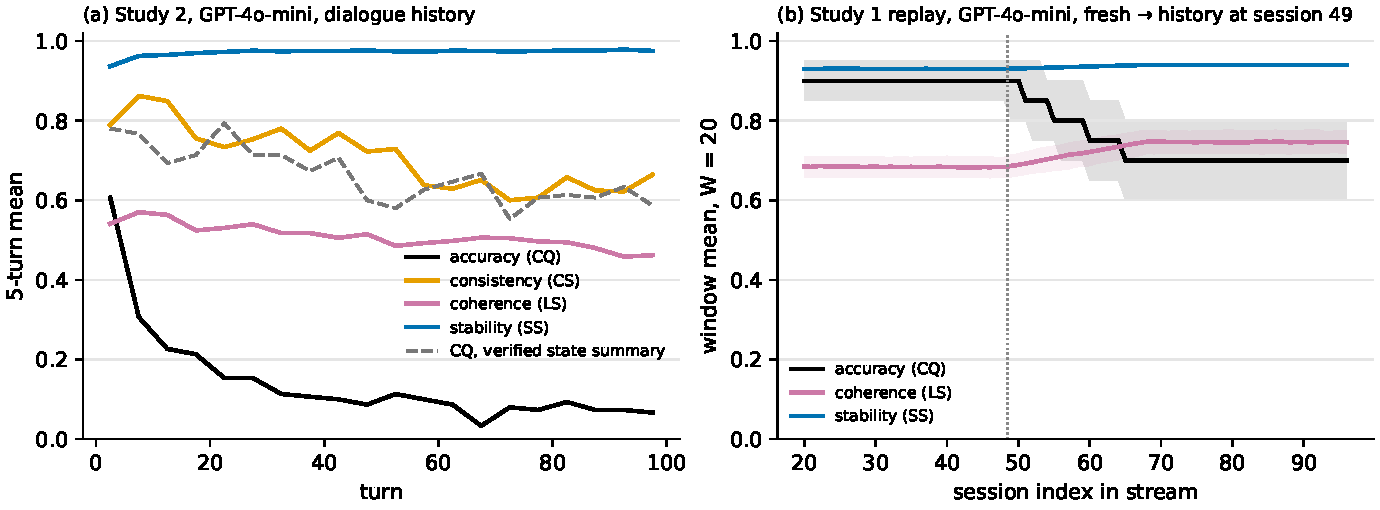
\includegraphics[width=\linewidth]{silent_metrics.pdf}
\caption{Quality metrics do not track accuracy. (a) Study 2, GPT-4o-mini,
dialogue history, means over 5-turn bins across 30 dialogues (descriptive);
the dashed line is accuracy under the verified state summary. CS is supported
by \silentCsSupport{} of 3,000 turns. (b) Post-hoc replay of Study 1 sessions:
median and 10--90\% band over 1,000 orderings of window means ($W=20$) when the
regime switches from fresh prefix to dialogue history at session 49.}
\label{fig:silent}
\end{figure}

\subsection{Calibrated single-stream detectors}

\paragraph{Study 1 replay (post hoc).}
In the replay, thresholds were calibrated on 2,000 permutation nulls with
family-wise $\alpha=0.05$ and validated on 2,000 disjoint nulls. Under that
control, the best detection rate for any metric, detector and strategy was
0.067 (Mistral-7B, CQ, sudden switch), with a median delay of about 44
sessions. No metric qualified as an early-warning candidate
(supplementary Table~S4).

\paragraph{Study 2, dialogue-history arm (confirmatory).}
The stationary dialogues that should serve as nulls themselves collapsed. For
CQ no grid value kept the null false-alarm rate at 5\% in most configurations,
so a threshold could not be calibrated at all. For the other metrics, detection
within 33 turns of the first change was at most 0.11. This is the core
difficulty of monitoring under accumulated history. The context-driven decline
starts at turn~1, before any detector has a reference period, and it is
present in exactly the streams that define normal behaviour.

\paragraph{Study 2, verified-state arm (exploratory, then validated).}
The control arm removes the background collapse and leaves only the scheduled
task drift, which makes it the cleanest test of the detectors themselves. On
GPT-4o-mini, with thresholds calibrated on the 12 stationary dialogues, CUSUM on
the window mean of CQ detected \ctrlScreenDetect{} drift dialogues within 33
turns at $W=20$. One reason is structural: the detectors ignore their first 20
window values, so at $W=20$ the earliest alarm falls near turn 40, after the
first change at turn 34. A simpler per-dialogue rule signals when the window
mean falls below $\mu_0-2\sigma_0/\sqrt{W}$ on three consecutive turns, with
$\mu_0$ and $\sigma_0$ taken from turns 1--30. It flagged accuracy in
\earlyCqSignal{} drift dialogues but also in \earlyCqNull{} stationary ones. LS
signalled in \earlyLsSignal{} drift dialogues, \earlyLsBefore{} of them before
accuracy, but also in \earlyLsNull{} stationary dialogues. Its apparent lead is
therefore not separable from noise.

These rules had been fixed after GPT-4o-mini trajectories were seen, so we
applied them unchanged to the unseen Llama-3 70B and Gemma 3 12B control arms
as a frozen validation. CUSUM detected \valLlamaDetect{} Llama drift dialogues
(median delay \valLlamaDelay{} turns) and \valGemmaDetect{} Gemma dialogues
(delay \valGemmaDelay{}), and neither model passed the frozen screen. The LS
rule signalled in \valLlamaLsSignal{} and \valGemmaLsSignal{} drift dialogues,
but also in \valLlamaLsNull{} and \valGemmaLsNull{} stationary dialogues. The
validation confirms that neither rule gives robust, model-general early
warning.

\subsection{Why single streams are underpowered}

The detector failures are not specific to our metrics. They follow from the
amount of information in one 100-turn stream. We simulated per-turn
correctness streams with pre-change accuracy 0.80 and a drop $\delta$ at turn
34 or 51. Each simulated turn aggregated $m$ independent dialogues. We used the
unchanged detectors and grids, calibrated thresholds on 12 null streams at a
5\% false-alarm target, and drew 300 drift streams per cell
(Table~\ref{tab:power}, Figure~\ref{fig:power}). A single stream reached 80\%
detection within 33 turns only for drops of about 0.5. The task drifts in our
data were 0.1--0.3. Aggregating six concurrent dialogues per turn brought the
detectable drop to 0.2, and 18 dialogues brought it to 0.1. Results were
similar for $W=10$ and $W=30$ and for larger calibration sets (supplement).

\begin{table}[t]
\centering
\caption{Simulated detector power: best unchanged detector, $W=20$, thresholds
from 12 null streams, 5\% false-alarm target. Columns 2--3: smallest accuracy
drop detected within 33 turns in at least 80\% of runs. Column 4: detection
rate for a drop of 0.2, averaged over both change points.}
\label{tab:power}
\small
\begin{tabular}{cccc}
\toprule
Dialogues per turn & Change at 34 & Change at 51 & Detection at $\delta=0.2$\\
\midrule
\inputtable{generated/table_power.tex}
\bottomrule
\end{tabular}
\end{table}

\begin{figure}[t]
\centering
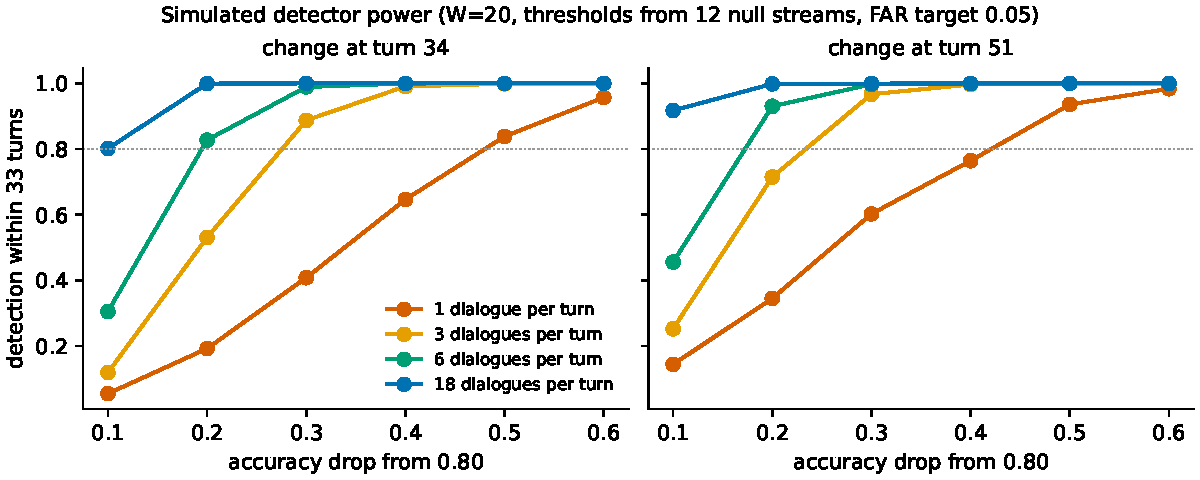
\includegraphics[width=\linewidth]{detector_power.pdf}
\caption{Simulated detection within 33 turns as a function of the accuracy drop
from 0.80 and the number of dialogues aggregated per turn ($W=20$, thresholds
from 12 null streams, 5\% false-alarm target). Left: change at turn 34; right:
change at turn 51. The dotted line marks 80\% detection.}
\label{fig:power}
\end{figure}

We then applied this idea to the control arms, which is exploratory. A CQ
CUSUM on the mean of the six dialogues of each scenario, with $W=20$, detected
all three drift scenarios in both validation models (\valLlamaAggDetect{} and
\valGemmaAggDetect{}). It raised no alarm in the two Llama stationary
aggregates but one in the two Gemma stationary aggregates (\valLlamaAggNull{}
and \valGemmaAggNull{}). Together with the GPT-4o-mini screen, this supports
aggregation across sessions as a promising direction. The small number of
scenario-level aggregates and the Gemma false alarm, however, preclude a
confirmatory claim.

\subsection{A baseline that could not fire}

In our generic ADWIN-everywhere baseline, ADWIN never alarmed in any analysis.
The cause was in our implementation. Its cut bound omitted the variance term of
\citet{bifet2007learning}, and without that term no difference of means in a
stream of at most 100 values in $[0,1]$ can exceed the bound. We re-ran every
affected analysis with a corrected ADWIN and with CUSUM in its place, as a
labelled sensitivity analysis. No conclusion changed: consistency and stability
still did not give early warning, so their earlier ``no warning'' result is now
genuinely tested rather than an artefact. Even the corrected ADWIN needed drops
of about 0.6 to detect reliably on 100-turn streams (supplement). The lesson is
general: a comparison against a generic baseline is only meaningful once the
baseline has been shown to fire on streams of the intended length.
